\chapter{绪论}
 % 简短的介绍
 

 \section{研究背景及意义}
 在中国改革开放和国际化进程的不断深入下,全社会对市场、对营销、对管理的态度发生了从无知到有知,从漠视到重视的巨大转变。时至今日,我们发现我们好像从来没有与世界的脉搏如此的接近过,同样,我们的企业和国家也从来没有如此深切的感受到全球化的竞争是如此的残酷。因为市场竞争的不断加剧,每个企业都在努力寻找着自己的核心竞争能力,以期望能在激烈的竞争中取得优势。但是,近年来,随着信息技术的广泛使用,众多行业的产品在价格、质量和服务上的差异越来越小,如何在如此激烈的市场竞争中领先对手,给当前的商业研究提出了新的要求,直复营销(Direct Marketing,DM)就是其中一个重要的研究方向。

 直复营销,即企业直接对客户进行营销的方式。在直复营销场景中,营销人员首先需要根据顾客的个人资料和其历史响应(购买)记录等信息,来构建关于客户的响应模型。然后,在每一次的营销活动中,再根据构建的响应模型来预测每一位目标客户可能会产生的期望收益,以此来决定应该对哪些目标客户进行这一次的营销行为。通常情况下,为了使每次营销活动能够产生的期望利润最大化,营销人员只会考虑那些可以给企业带来正向(非零)期望利润的客户进行营销\citep{王广宇2013客户关系管理}。直复营销的具体过程如图$\ref{fig:直复营销示意图}$所示。
	\begin{figure}[htbp]
	\centering
	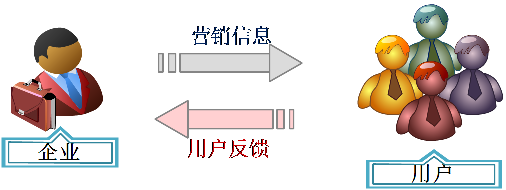
\includegraphics[width=0.5\textwidth]{直效营销示意图}
	\caption{直复营销场景示意图}
	\label{fig:直复营销示意图}
	\end{figure}

近年来,越来越多的机器学习技术被运用到直复营销领域中。最开始,研究人员通过使用经典的分类模型,以营销决策的低错误率为学习目标,来解决上述直复营销问题。但是,因为在该场景中,不同的错误分类所带来的代价是不同的,所以传统的分类算法有很大的局限性。基于这个问题,后续出现很多基于代价敏感(cost-sensitive)学习的方法,这些方法以追求最小分类代价为目标,取得了比传统分类算法较好的性能。

但是,以上这些方法只能最大化单个决策的收益,而在像直复营销这类应用场景中,随着时间的推移是需要不断做出决策的,因此属于序贯决策问题。所以,在进行营销决策时,不仅需要考虑单个决策的成本和收益,还要考虑到随着时间的推移,其对后续决策结果可能产生的影响。比如:在某一次营销活动时,某个客户所产生的预期收益可能会大于营销成本,但是,这次的营销可能会让该客户在之后的营销中产生更大的收益。所以,在某些时刻,为了能让客户在以后的时间里能产生更大的收益,营销人员可能要牺牲短期的利润,以达到最大化客户生命周期价值的目的。而这对于基于监督学习或者非监督学习的机器学习算法很难办到的,

强化学习(Reinforcement Learning, RL)是机器学习的重要组成部分,主要用于解决序贯决策问题。其主要学习过程如图$\ref{fig:强化学习过程}$所示:通过智能体(Agent)不断地与环境(Environment)进行交互,并从环境反馈的延迟回报中学习状态与行为之间的映射关系,以使得可以达到累积奖赏最大化。在以上过程中,可以发现:因为强化学习在学习过程中考虑到了延迟回报,并且只关心当前采取什么行为可以使整个任务序列达到累积奖赏最大化,所以,强化学习技术可以很好的解决直复营销场景中在序列决策之间存在相互影响的问题,同时还可以达到最大化客户生命周期价值的目标,这也是本文选择使用强化学习解决直复营销决策问题的出发点。特别地,本文主要关注基于值函数的强化学习算法。
\begin{figure}[htbp]
\centering
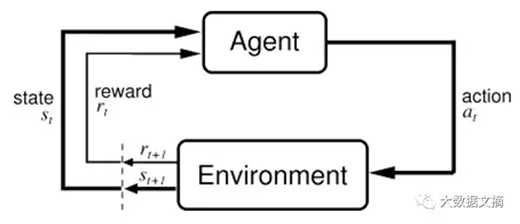
\includegraphics[width=0.6\textwidth]{强化学习过程}
\caption{强化学习的交互过程}
\label{fig:强化学习过程}
\end{figure}

强化学习是从控制工程、心理学和运筹学等相关学科发展起来的。在上个世纪八十年代到九十年代,强化学习的理论基础研究取得了突破性进展,随后越来越多的被应用于工业控制、作业调度和机器学习等领域。比如,Macek等人将强化学习技术应用机器人躲避障碍物,Tesaruo等人结合神经网络将强化学习应用与西洋双陆棋中。近年来,DeepMind团队将深度强化学习技术结合蒙特卡罗树搜索,研发的AlphaGo大胜世界围棋冠军李世石和柯洁,从而在学术界和工业界再一次掀起了研究强化学习的高潮。

虽然强化学习的研究和应用已经取得了突破性的进展,但是由于强化学习问题本身的复杂性,加之不同应用场景的特殊性,强化学习算法在实际应用中任然面临一定的困难,包括:

1)在值函数逼近上,面对大规模的状态空间和行为空间,仍然存在收敛速度慢和精度不高的问题。训练速度较慢,而传统的随机采样方法不能高效的利用数据。

2)强化学习与场景的结合更加紧密,需要根据不同场景特点进行相应的算法改进。

3)大部分的应用场景都存在环境的部分可观测问题,此时为了更好逼近值函数,需要借助大量的专家领域知识。

\section{研究现状}

\subsection{直复营销的研究现状}
在机器学习领域,针对直复营销场景的研究,主要分为三种:

基于传统的分类算法。在文献\citep{alam2012actionable, ngai2009application, wong2005mining, coussement2015improving}中作者分别使用逻辑回归、线性二次判别分析法、朴素贝叶斯、神经网络、决策树以及KNN等算法,对用户的响应模型进行建模,研究各类算法在直复营销中的应用效果,并在模型的可解释性和准确性方面给出了权衡建议。但是,这类算法在学习的时候假设误分类的代价是相同的,而在实际的直复营销应用中对不同客户误分类给企业所带来的损失是不同的,所以使用传统的分类算法必然会带来一定的局限性。

基于代价敏感的分类算法。针对以上传统分类算法在应用中存在的问题,众多学者开发出了代价敏感的分类算法。文献\citep{bahnsen2015example}中,Bahnsen等将误分类代价加入到决策树的构建中,提出了最小代价决策树,并将其应用在了信用卡欺诈检测,信用评分和直接营销场景中,取得了比传统分类算法更好的效果。在文献\citep{cui2012cost}中,Cui等通过贝叶斯网络本身含有的先验概率计算出事例属于每个累的概率,然后根据经验风险公式直接对其进行代价敏感分类,用于解决直邮营销场景下的代价敏感的问题。这些基于代价敏感的分类算法虽然考虑到了误分类的不同代价问题,但是,在进行决策时每个决策点都是独立的,无法捕捉到直复营销序列决策中的相互影响,进而也就无法达到最大化长期收益的目的。相关的应用研究还有\citep{migueis2017predicting,zakaryazad2016profit,hu2015cost}

基于强化学习的方法。因为强化学习通过考虑决策序列中的延迟影响进而可以最大化长期收益,可以很好的解决直复营销场景中不同营销时刻之间的的影响,以达到最大化客户生命周期价值的目的。近年来已经开始有学者尝试使用强化学习技术来解决营销中的相关应用问题。为了解决独立决策点的问题,Pednault等人\citep{pednault2002sequential}首次将强化学习技术用于解决直复营销问题,并对如何仿真等给出了解决方案。\citep{kim2009new}等人针对在直复营销中的客户流失问题,提出将客户的流失概率作为约束条件,并试图在给定的阈值下对其进行控制的强化学习方法。Silver等人\citep{silver2013concurrent}提出了一种基于时间差分学习的并行强化学习框架。通过该框架可以并发的实现企业与客户之间的交互,并且通过模拟器分别在非自举(Non-bootstrappig)、非在线(Non-online)和非序列化(Non-sequential)三个方面进行了模型的对比评估,得到了在高并发的序列化问题中,应该考虑使用进行自举、在线学习以及使用序列化的强化学习方法的结论。但是,以上这些算法都没有考虑在直复营销过程中的存在可变时间间隔问题,这将是本文第三章的研究内容。在深度强化学习放面。Tkachenko等人\citep{tkachenko2015autonomous}使用了深度强化学习解决直效营销中的问题,即使用Q-learning的方法训练一个深度神经网络来学习客户的状态和营销行为之间的关系,同时,该文章使用Recency-Frequency-Monetary指标参数化客户状态空间,实现了顾客响应率和顾客花费金额两方面的显著提高。但是,该方法没对直销营销中的部分可观测问题进行分析。

\subsection{强化学习的研究现状}

\paragraph{发展阶段}
强化学习的发展过程大概可以分为三个阶段。

第一阶段是1998年以前,这一阶段形成了强化学习基本理论框架,学者们关注和发展的最多的算法是基于表格型的强化学习算法,包括值迭代和策略迭代。代表性的工作是强化学习鼻祖Richard将其专刊装订成书,这标志着强化学习发展成为机器学习领域的一个重要分支。该书《Reinforcement Learning: An introdcution》是强化学习领域的经典著作,第一次系统而全面的介绍了强化学习的相关理论知识,至今仍然被广大的教育机构和强化学习爱好者作为强化学习的经典教材(该书最新电子版可在网上免费获取\footnote{http://incompleteideas.net/book/bookdraft2017nov5.pdf}),需要注意的是,这期间还出现了强化学习代表性算法Q-learning\citep{watkins1992q}和Sarsa\citep{rummery1994line}。

第二阶段是1998年到2013年,这一阶段基于直接策略搜索的强化学习方法得到了深入研究和发展。自从Williams在其论文\citep{williams1992simple}中提出直接对Reinforce算法的策略梯度进行估计这一方法后,出现了各种改进方法,如:GPOMDP\citep{baxter2001infinite}、PEGASUS\citep{neumann2005reinforcement}以及与值函数结合的Actor-Critic算法\citep{konda2000actor}等。

第三阶段是2013年以后,随着深度学习的发展,这一阶段出现了深度强化学习算法。代表性的工作是DeepMind团队提出了DQN(Deep Q Network)算法并将其成功应用在雅达利(Atari)游戏中\citep{mnih2013playing},之后无数的学者对其进行了改进研究,但是
大部分都应用在机器人和游戏中。
其中,最具轰动性的事件当属在2016年和2017年,谷歌的AlphaGo利用深度强化学习算法连续两年分别击败了世界围棋冠军李世石和柯洁。

\paragraph{研究热点}
但是,目前强化学习在实际应用中仍然存在维度灾、收敛速度慢、时间信度分配等问题,其中维度灾是指在大空间和连续问题中,强化学习无法在有限的空间和时间内学习到一个合理的解决方案,而收敛速度慢又与强维度灾有着密切的关联,所以解决维度灾问题对强化学习的应用起到了十分重要的作用。近年来,众多研究者主要集中于利用函数逼近的方法解决此问题,而函数逼近方法又可以分为参数化函数逼近方法和非参数化函数逼近方法。

参数化函数逼近方法又可以分为线性函数逼近和非线性函数逼近两种方法。其中在线性函数逼近中,基函数的形式和参数个数需要提前制定,往往会限制函数的逼近能力。该方法最早是由Samuel在1967年提出,并将其应用于西洋跳棋的系统设计中\citep{samuel1959some}。1988年,Sutton提出将线性函数逼近法与带有资格迹的时间差分(Temporal Difference, TD)方法相结合,然后使用梯度下降求解近似值函数的方法后\citep{sutton1988learning},掀起了线性函数逼近法研究的热潮,相继出现了最小二乘时间差分(Least Squares Temporal Difference, LSTD)算法\citep{bradtke1996linear}、离策略(Off-policy)函数逼近方法\citep{precup2001off}、以及梯度时间差分(Gradient Temporal Difference, GTD)学习算法\citep{sutton2009convergent}等,其中GTD解决了离策略TD学习算法的不稳定问题,且具有较低的时间负责度\citep{sutton2009convergent}。

非线性函数逼近方法中的函数逼近器是关于参数的非线性函数,如神经网络。虽然该方法具有很强的表征能力,但是容易陷入局部最优,且收敛性难以保证。1995年Bertsekas等\citep{bertsekas1995neuro}利用前向神经网络逼近强化学习中的值函数,取得了相比线性逼近较好的结果,但是往往会出现不稳定不收敛的情况。直到DeepMind团队于2013年提出了DQN网络,才使的这一问题得到有效解决。在DQN网络中,通过在训练过程进行经验回放\citep{mnih2013playing}和单独设立目标网络\citep{mnih2015human}这两种改进方法,打破了数据之间的关联性,使的神经网络的训练过程收敛且稳定,并且在游戏中取得了令人振奋的表现。从此以后,彻底掀起了学术界和工业界研究深度强化学习的热情。2015年DeepMind团队又提出了Double DQN模型,在该模型中为了克服Q-learning本身固有的缺点——过估计(Overestimate),将动作的选择和动作的评估分别使用不同的值函数来实现。除此以外,深度Sarsa、A3C(Asynchronous Advantage Actor-Critic)、DDPG(Deep Deterministic Policy Gradient)等一些列有影响力深度强化学习模型相继被提出。

非参数化函数逼近法,并不是没有任何参数的函数逼近,而是指参数个数和基函数的形式并非固定,完全由样本决定,因此具有更大的灵活性和表征能力,但是当样本量很大时,将会带来更大的计算开销。非参数化函数逼近模型主要有基于高斯过程和基于核方法的值函数逼近模型。其中,基于核方法的研究相对较多,如基于核的强化学习函数逼近方法\citep{ormoneit2002kernel}、基于核的最小二乘TD方法(Kernel-based Least Squares TD, KLSTD)\citep{xu2005kernel}、基于最小二乘的策略迭代算法等(Kenel-based Least Squares Policy Iteration, KLSPI)\citep{xu2007kernel}等。

\paragraph{发展趋势}
强化学习正在飞速发展,从当前的研究工作中可以判断强化学习的发展具有如下趋势:1)强化学习与深度学习的结合会更加紧密。2)强化学习与领域知识的结合更加紧密,特别是在重塑回报函数的方向上。3)强化学习的理论分析会更加全面、具体,算法性能会更加稳定和高效。本文的研究工作正是从前两个方面展开的。

\section{主要研究内容}

\section{本章小结}


